%---------------------------------------------------------------
\chapter{Well-specified models experiments}
\label{chap:well_specified}
%---------------------------------------------------------------

Having already had all the necessary theoretical basis passed, it is time to go directly to the practical part. The experiments will be conducted directly on the three different SSMs described in detail below. Among the models will be both linear and non-linear. Such indicators as efficiency, performance, and robustness of the following algorithms will be compared: KF, EKF, particle filter, and the modification of particle filter with ABC approximation and automatic kernel tuning.

Within the framework of this chapter the experiments will be conducted on well-specified correct models. Also, importantly, one of the main tasks in this chapter is to consider the tracking performance of the approximate filtration with adaptive kernels and how close it is to the performance of a regular particle filter using the correct model.

The mean square error (MSE) will be used as a performance indicator, which is calculated as follows:

\begin{equation}
    \begin{aligned}
        M S E &=\frac{1}{t} \sum_{\tau=1}^t\left(\hat{x}_\tau-x_\tau\right)^2 \\
        &=\frac{1}{t} \sum_{\tau=1}^t\left(\sum_{i=1}^N W_\tau^{(i)} x_\tau^{(i)}-x_\tau\right)^2,
\end{aligned}
\end{equation}

\noindent which is residual sum of squares resulting from comparing the predictions \(\hat{x}_t\) with the ground truth \(x_t\). This is one of the most popular metrics for scoring how close the model's outputs are to ground truth desired values. It is worth recalling that in the case of the ideal model, the MSE value will be zero.

\section{Technical prerequisites}
All of the following experiments were performed on the following laptop computer MacBook Pro (Retina, 15-inch, Mid 2014). All experiments were performed repeatedly to obtain sufficiently representative results, as well as to smooth out, if possible, the technical limitations associated with the computing power and technical limitations of the available device.

As for the experiments themselves and the required dependencies, the programming language Python3.9 and the following dependencies were used:
\begin{itemize}
    \item NumPy v.1.21.3 - primarily for mathematical operations
    \item SciPy v.1.7.1 - in most cases only the \textbf{stats} module containing a huge number of statistical functions
    \item Matplotlib v.3.4.3 - responsible for everything related to visualization
\end{itemize}

\section{Example 1: Power growth model}
The first example should, in fact, prove that the performance of the proposed approximate filter with adaptive kernel should be quite close to the performance of the standard bootstrap particle filter or, on the contrary, disprove this statement. It is worth recalling that unlike particle filters, approximate filters do not require full knowledge of the measurement model, i.e. it is sufficient for them to work with equations without noise terms.

On the agenda is a popular problem rooted in such fields as ecology and epidemiology, referred to as the exponential growth model. But let's consider a slightly modified version of the problem, replacing the exponential function with a exponentiation (power)  and call it the power growth model (PGM). The PGM has the following form:

\begin{equation}
\begin{aligned}
    y_t &= k + \mu_t + \varepsilon_t, \\
    \mu_t &= \mu_{t-1}^{1+\nu_{t-1}} + \xi_t, \\    
    \nu_t &= \rho\nu_{t-1} + \zeta_t,
\label{eq:pgm_equations}
\end{aligned}
\end{equation}

\noindent where \(\rho\in[0,1]\) is the "discounting" factor and \(k\) is the drift. We either know both of these variables or we have to estimate them appropriately. As can be seen, the process is nonlinear and very sensitive to combinations of \(\nu_t\) and \(\mu_t\) values. It is enough to keep the inappropriate combination for a while and the process will explode. 

The next step is to make an appropriate state-space model from the above equations:

\begin{itemize}
    \item State evolution model:

    \begin{equation}
        x_t = \begin{bmatrix} \mu_t \\ \nu_t \end{bmatrix}
        = 
        \begin{bmatrix} \mu_{t-1}^{1+\nu_{t-1}} \\ \rho\nu_{t-1} \end{bmatrix}
        + w_t,
   \end{equation}    
    where
    \begin{equation}
        w_t \sim (0, Q) \quad \text{with} \quad Q = \left[\begin{array}{cc}
            \xi_t^2 & 0 \\
            0 & \zeta_t^2
        \end{array}\right],
   \end{equation}

    \noindent that is nonlinear, will require linearization if the EKF is used.
    \item Measurement model:
    \begin{equation}
        \begin{aligned}
    y_t &= H_t x_t + B_t u_t + \varepsilon_t \\
    &= [1, 0]
    x_t + k + \varepsilon_t.
        \end{aligned}
        \label{eq:pgm_measurement_model}
    \end{equation}

    \noindent which does not require linearization, because it is already linear.
\end{itemize}

Since the EKF is one of the filters used in the experiment, it is necessary to linearize the equation of state, i.e., to determine the derivative of the two-dimensional function \(f\left(\cdot\right)\) - the first vector on the right-hand side:

\begin{equation}
F_t =
\begin{bmatrix}
(\nu_{t-1} + 1) \mu_{t-1}^{\nu_{t-1}} &
\mu_{t-1}^{1+\nu_{t-1}} \ln \mu_{t-1} \\
0 & \rho
\end{bmatrix},
\end{equation}
\noindent that is in the state prediction the \emph{nonlinear equation} will be used to predict \(\hat{x}_t^-\) and the time-varying \emph{matrix} \(F_t\) to predict \(P_t^-\). As for the update step, no linearization is required and the linear measurement equation will be used.

Since this chapter assumes that the model is correct specified, the noise terms belong to the following distributions:

\begin{equation}
\begin{aligned}
\varepsilon_t &\sim \mathcal{N}(0, 10^2), \\
\xi_t &\sim \mathcal{N}(0, 0.1^2), \\
\zeta_t &\sim \mathcal{N}(0, 0.01^2),
\end{aligned}
\end{equation}

\noindent the noise variables \(\varepsilon_t\), \(\xi_t\) and \(\zeta_t\) are independent and identically distributed. It is clear that under the following conditions, there is the  Gaussian measurement model \(g_t\), and also, the measurements \(y_t\) are corrupted by Gaussian noise. It can reasonably be expected that both EKF and PF will perform exceptionally well since all necessary assumptions are met.

It is also important to add that since the second equation (\ref{eq:pgm_equations}) has a mathematical operation with raising a number to a degree, in order to avoid numerical errors during filtering, a couple of mathematical tricks have been added to the function that deals with particle evolution, such as discarding particles that lead to invalid values, etc., thus ensuring that SMC filters work normally. Unfortunately, given the architecture of the EKF filter, which cannot select from many particles, no modifications have been added to it. Thus, one should consider that the EKF filter may generate invalid values on one of the iterations.

\paragraph*{Initialization} The initial parameters are \(x_0=[100,0] \), \(k=2\), \(\rho=0.9\), the length of the series is 500 samples. The EKF filter and three variants of SMC filters were compared. Among the SMC filters are the bootstrap PF, the ABC filter with Gaussian kernel, and the ABC filter with Cauchy kernel. The inference started at the following parameters: the prior state values for EKF are \(x_0 = [0, 100]\) and \(P^{-} = 10 I_{2 \times 2} \), where \(I_{2 \times 2}\) denotes the identity matrix of rank 2. For SMC filters, an initial set of 1000 particles for nonlinear states is randomly sampled from \(\mathcal{N}([100,0],
\begin{bmatrix*}
0.1^2 & 0 \\
0 & 0.01^2
\end{bmatrix*}
) \) and used in all SMC filters. Unlike the PF filter, the ABC filters lack the full knowledge of the measurement model. The ABC filters setting are the HPR value \(p = 0.95\) and covers \(90\%\) of pseudo-measurements. Each SMC filter performs a multinomial resampling at the beginning of each time step. An experiment with 100 independent repetitions was conducted to obtain representative results.

\paragraph*{Charts and analysis}
Accordingly, after 100 experiment runs of all filters, each time on newly generated data, the following results were obtained, presented in the graphs below. Figure \ref{fig:pgm_mse_boxplot_normal} shows the statistics of the final MSE values in the form of box plots. As one would expect, with full knowledge of the measurement model, the EKF and PF filters showed quite acceptable and unambiguously best results among the other filters. It was quite expected that PF would prove to be a fairly stable filter, even it can be seen that its results are slightly, but still better than those of EKF. Just the same, it can be observed that with a sufficient number of particles, the PF is more accurate than the EKF, although computationally more expensive. The stability of the filter can also be proved by the fact that the value from the Table \ref{table:pgm_mse_normal}, which shows the average of final MSE values after 100 experiment runs, is not very different from the median value shown on the box plot. Also, compared to standard approximation methods such as EKF, the PF's main advantage is that it does not rely on any local linearization technique. As for ABC filters, it can be stated that their results against the background of EKF and PF look worse, but not much, especially given the lack of accurate knowledge of the measurement model. It can be seen that the ABC filter operation in the context of this model is not quite sensitive to the choice of kernel. So, for example, from Figure \ref{fig:pgm_mse_boxplot_normal}, one can see that the ABC filter with the normal kernel performed slightly better for tracking both state variables \(\mu\) and \(\nu\). Also, if one looks at the table \ref{table:pgm_mse_normal} with the averaged values after all 100 experiment runs, one can observe the same, that the results are almost identical for both ABC filters, but still, the filter with the normal kernel shows a slightly better performance.

\begin{figure}[!ht]
\centering
\caption{(PGM, Normal noise) Box plots showing final MSE values for both state variables \(\mu\) and \(\nu\) of 100 repeated experiments. The boxes show medians, upper and lower quartiles. The length of the whiskers is defined as 1.5 times the interquartile range. The outliers are not displayed.}
\subfloat{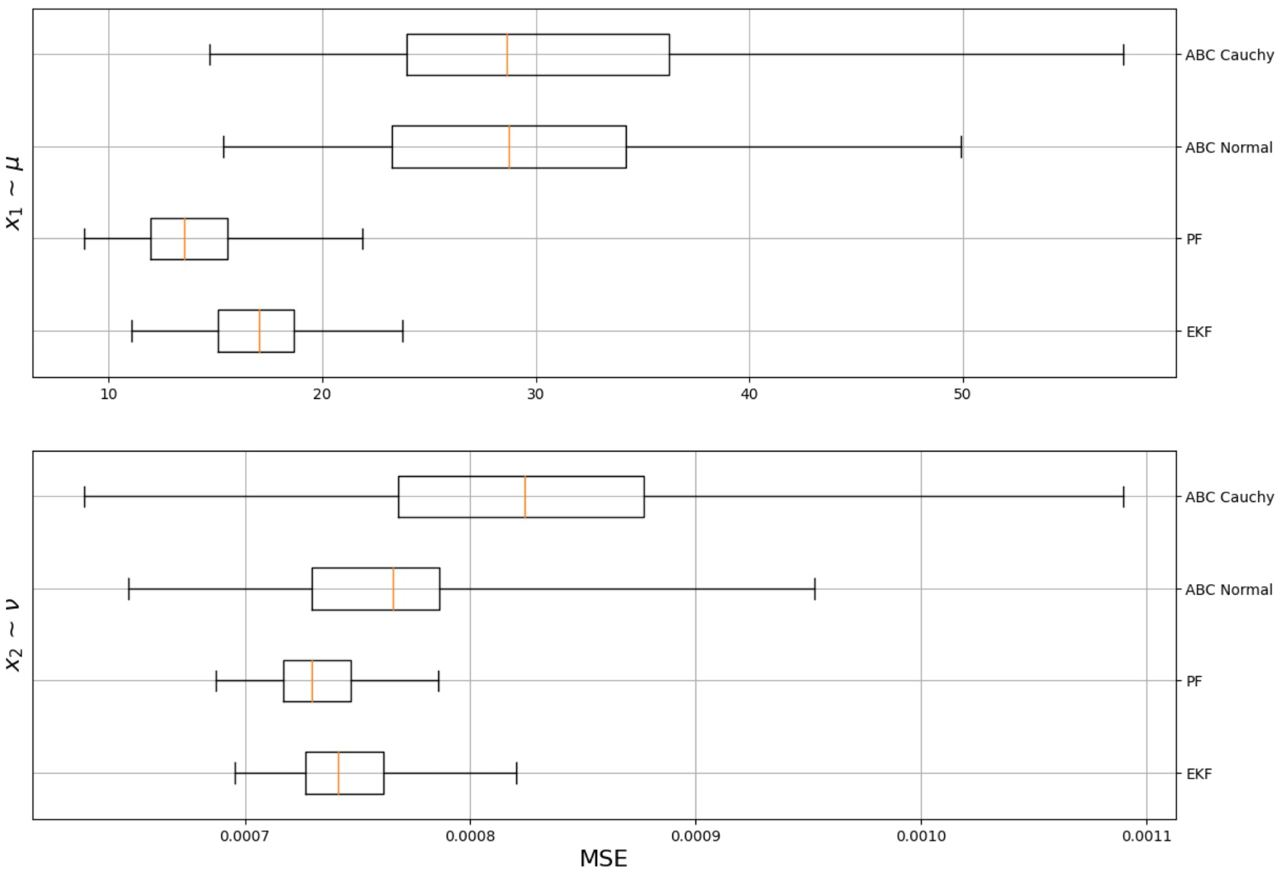
\includegraphics[width=0.9\columnwidth, height=\textheight,keepaspectratio]{figures/pgm/mse_boxplot_normal.jpg}}
\label{fig:pgm_mse_boxplot_normal}
\end{figure}

\begin{table}[h!]
\centering
\begin{tabular}{ |p{4cm}|p{4cm}|p{4cm}|}
 \hline 
  & \(\mu\) & \(\nu\)\\
 \hline \hline
 EKF & 17.029    & 7.435e-04  \\
 PF  &   13.840  & 7.319e-04 \\
 ABC Normal & 29.347 & 7.646e-04\\
 ABC Cauchy & 30.963 & 8.274e-04\\
 \hline
\end{tabular}
\caption{(PGM, Normal noise) The final MSE values for both state variables \(\mu\) and \(\nu\) averaged over 100 runs}
\label{table:pgm_mse_normal}
\end{table}

Another indicator worth paying attention to is shown in Figures \ref{fig:pgm_measurement_noise_normal} and \ref{fig:pgm_abc_scales_evolution_normal}. The first Figure shows the implementation of the measurement noise \(\varepsilon_t\) in the final experiment run, and the second shows the scale settings of the ABC filter kernels in the final experiment run. Basically, both cases show the same \(\varepsilon_t\) evolution characteristics. Clearly, there are some minimal differences, but this is a property of the kernels themselves.


\begin{figure}[!ht]
\centering
\caption{(PGM, Normal noise) One particular normal noise realization \(\varepsilon_t\). Relative frequency histogram and box plot. The box shows the median, upper and lower quartiles. The length of the whiskers is defined as 1.5 times the interquartile range. Dots closer to the edges of the box represent outliers.}
\subfloat{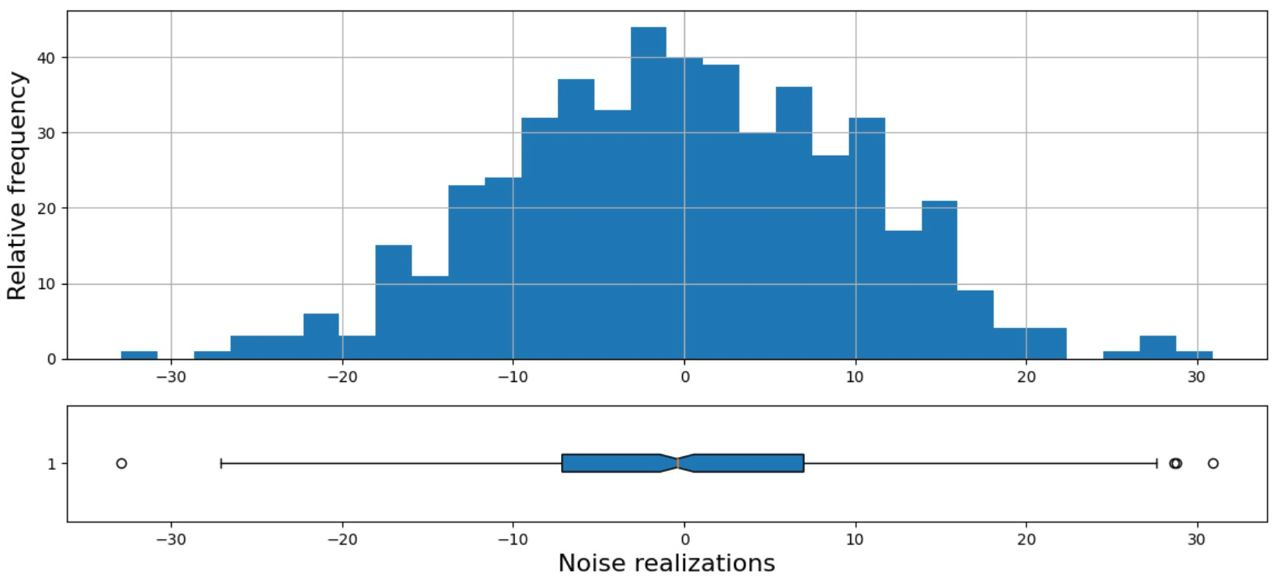
\includegraphics[width=0.9\columnwidth, height=\textheight,keepaspectratio]{figures/pgm/measurement_noise_normal.jpg}}
\label{fig:pgm_measurement_noise_normal}
\end{figure}

\begin{figure}[!ht]
\centering
\caption{(PGM, Normal noise) The top two graphs show the one particular evolution of the normal and Cauchy scales \(\varepsilon_t\), respectively. The bottom one represents the normal noise realizations.}
\subfloat{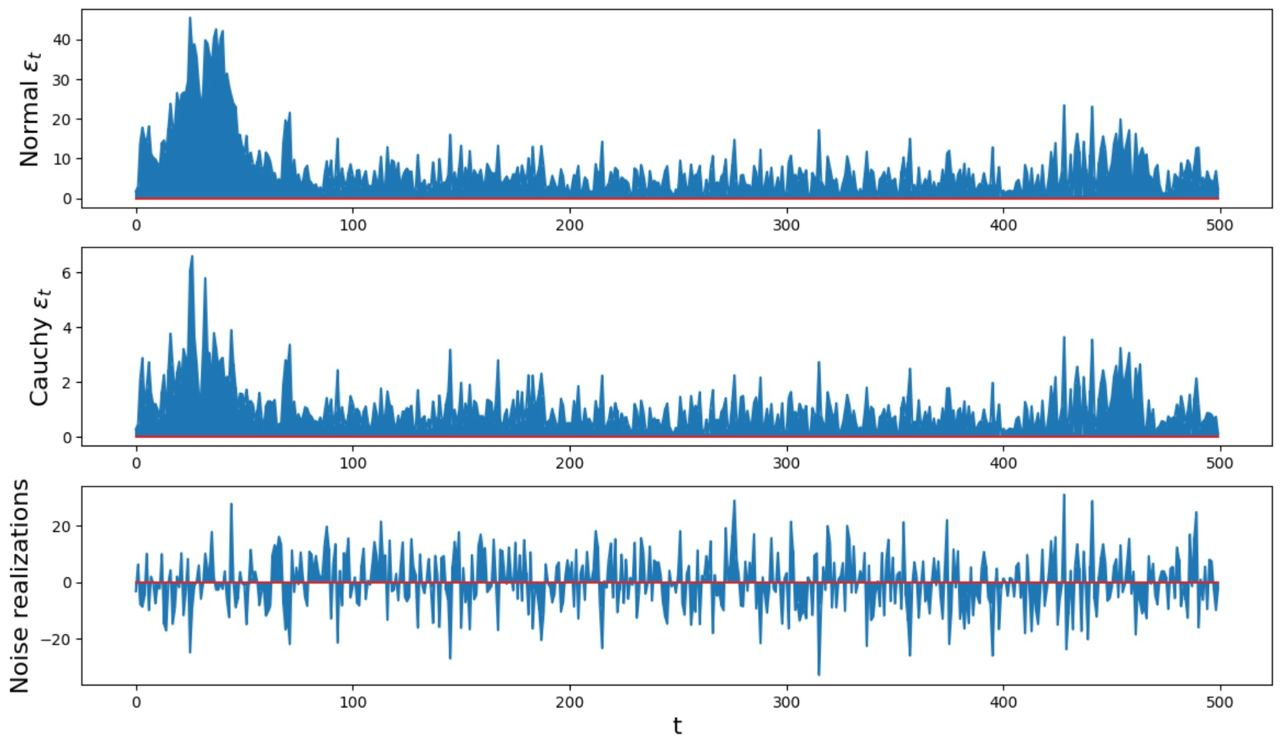
\includegraphics[width=0.9\columnwidth, height=\textheight,keepaspectratio]{figures/pgm/abc_scales_evolution_normal.jpg}}
\label{fig:pgm_abc_scales_evolution_normal}
\end{figure}

In general, based on the example of this experiment, one can say that all the filters showed pretty good results with the obvious favorites. Considering that ABC filters do not require the measurement generating model to be probabilistic, also showed good results. In this example, the ABC filter with the normal kernel stands out slightly better, but overall, both ABC filters showed almost identical good results.

\section{Example 2: Constant velocity model}
Next in line is a fairly popular and well known constant velicty model (CVM). The model is absolutely linear and its purpose is to filter the position of an object moving on the surface, i.e. in 2D. The CVM has the following form:

\begin{equation}
    \begin{aligned}
        x_{1,t} &= x_{1,t-1} + v_{x_1,t} dt + w_{x_1,t}, \\
        v_{x_1,t} &= v_{x_1, t-1} + w_{vx_1, t},
    \end{aligned}
    \label{eq:cvm_equations}
\end{equation}

\noindent where the first equation characterizes the current position of the object in both axes, and the second equation characterizes the velocity of the object at a given time. Consider that the velocity is the same and its changes are caused only by noise. Only position measurements in both axes are available in 1 second time steps. An example for one axis looks like this:

\begin{equation}
\begin{aligned}
    y_{1,t} &= x_{1,t} + \varepsilon_{y_1,t}.
\end{aligned}
\label{eq:cvm_measurement_equation}
\end{equation}

All the same filters will be used for this model as for the previous one, except that this model is absolutely linear, so KF will be used instead of EKF. It is time to make the appropriate SSM from the above equations:

\begin{itemize}
    \item State evolution model:
    
    \begin{equation}
        x_t = \begin{bmatrix}
        x_{1,t} \\ 
        x_{2,t} \\ 
        v_{x_1,t} \\ 
        v_{x_2,t}
\end{bmatrix}
        = \begin{bmatrix}
       1 & 0 & dt & 0 \\
       0 & 1 & 0 & dt \\
       0 & 0 & 1 &  0 \\
       0 & 0 & 0 &  1 
    \end{bmatrix} x_{t-1} + w_t,
   \end{equation}   
   
    \noident where

    \begin{equation}
        w_t \sim (0, Q_t) \quad \text{with} \quad Q = q^2 \cdot
    \begin{bmatrix}
        \frac{dt^3}{3}    & 0                 & \frac{dt^{2}}{2}  & 0  \\
        0                 & \frac{dt^3}{3}    & 0                 & \frac{dt^{2}}{2} \\
        \frac{dt^{2}}{2}  & 0                 & dt                & 0 \\
        0                 & \frac{dt^{2}}{2}  & 0                 & dt
    \end{bmatrix}.
   \end{equation}

   \item Measurement model:

    \begin{equation}
    \begin{aligned}
    y_t &=  \begin{bmatrix}
        1 & 0 &0 & 0 \\
        0 & 1 &0 & 0
    \end{bmatrix} x_t + \varepsilon_t,
        \end{aligned}
        \label{eq:cvm_measurement_model}
    \end{equation}
    \noident where
    \begin{equation}
        \varepsilon_t \sim (0, R_t) \quad \text{with} \quad R =
    r^{2}\cdot
    \begin{bmatrix}
        1 & 0 \\
        0 & 1
    \end{bmatrix}.
   \end{equation}
    
\end{itemize}

Just like last time, based on the assumption that the model is correctly specified, the noise terms belong to following normal distributions:

\begin{equation}
\begin{aligned}
w_t &\sim \mathcal{N}(0, Q_t), \\
\varepsilon_t &\sim \mathcal{N}(0, R_t).
\end{aligned}
\end{equation}

\paragraph*{Initialization} The initial parameters are \(x_0=[0,0,1,-1] \), \(dt=1\), \(r=3\), \(q=\sqrt{5}\), the length of the series is 300 samples. Accordingly, the KF filter and three other variations of SMC filters will be compared. Just like in the previous example, the SMC filters include bootstrap PF and two ABC filters with normal and Cauchy kernels. The initial parameters for the KF filter are \(x_0 = [1,1,1,1]\) and \(P^{-} = 10000 I_{4 \times 4} \). As for the SMC filters, the following setup is provided: an initial set of 1000 particles is randomly sampled from \(\mathcal{N}\left(\left[1,1,1,1\right], 10 I_{4 \times 4} \right)\) and used in all SMC filters. For the ABC filters, the same settings are left as in the previous example: the HPR value \(p = 0.95\) in order to cover \(90\%\) of pseudo-measurements. An experiment with 100 repetitions was conducted to obtain representative results.

\paragraph*{Charts and analysis} 
To begin with, it is worth taking a look at the statistics of the final MSE values. Figure \ref{fig:cvm_mse_boxplot_normal} presents the statistics of the final MSE values of 100 repeated experiment runs in form of box plots. The table \ref{table:cvm_mse_normal} shows the averaged MSE values after 100 experiment runs for all filters used.

According to the results in Figure \ref{fig:cvm_mse_boxplot_normal}, it can again state that globally the KF and PF filters succeeded best in tracking all 4 state variables. As it is already known from theoretical part that KF is the best possible linear estimator, and this is confirmed in this example, because it showed excellent results. Almost identical, but a little worse results were shown by PF, although it succeeded a little better with tracking \(v_2\). The ABC filters also showed good results in tracking state variables. According to box plots, it may seem that ABC filter with normal kernel performs better than similar filter with Cauchy kernel. Given that the ABC filter with Cauchy kernel has the most distant right whisker, i.e., the maximum error value, it can be concluded that, despite the good performance, it still sometimes made quite strong errors compared to the others. 
But if we look at the average of the final values for all experiment runs in the Table \ref{table:cvm_mse_normal}, one can see that the final averaged MSE values of both ABC filters are quite close. But it should admitted that the results of the filter with the normal kernel are slightly, but still better.

\begin{figure}[!ht]
\centering
\caption{(CVM, Normal noise) Box plots showing final MSE values for all state variables $x_1$, $x_2$, $v_1$ and $v_2$ of 100 repeated experiments. The boxes show medians, upper and lower quartiles. The length of the whiskers is defined as 1.5 times the interquartile range. The outliers are not displayed.}
\subfloat{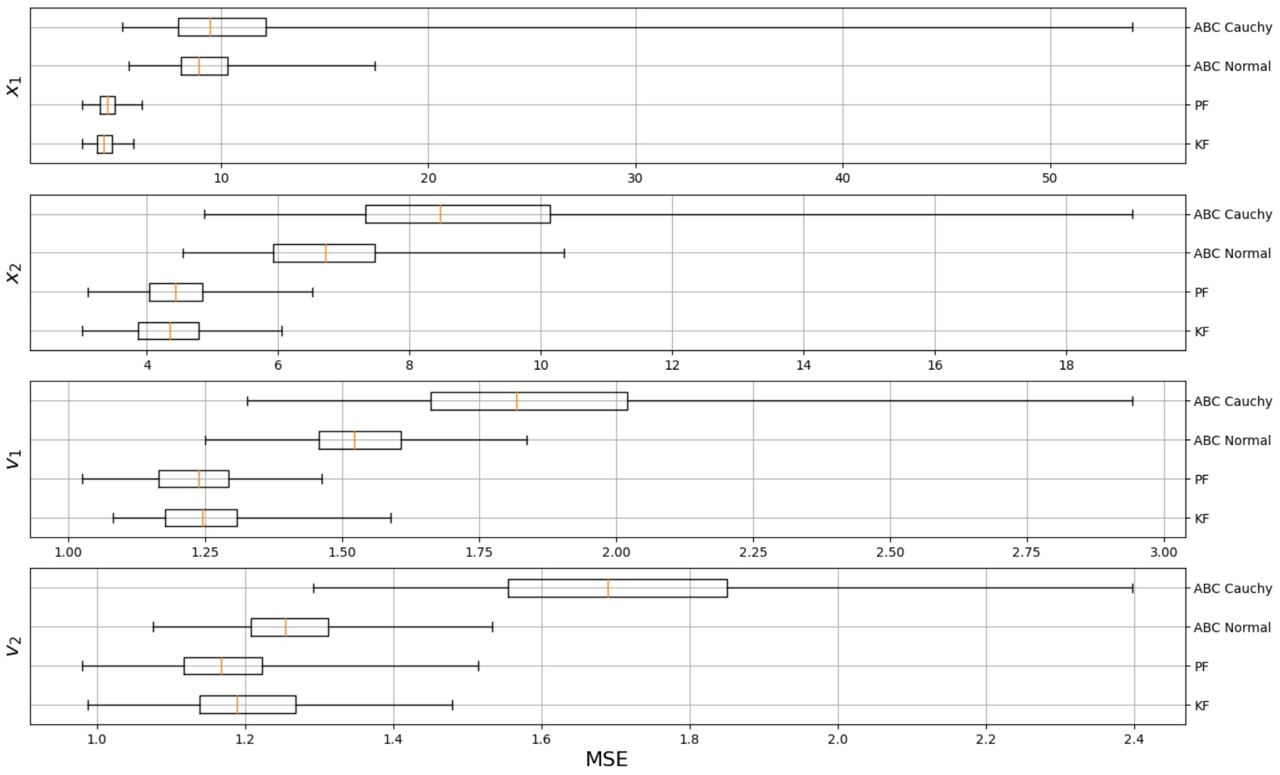
\includegraphics[width=0.9\columnwidth, height=\textheight,keepaspectratio]{figures/cvm/mse_boxplot_normal.jpg}}
\label{fig:cvm_mse_boxplot_normal}
\end{figure}

\begin{table}[h!]
\centering
\begin{tabular}{ |p{2cm}|p{2cm}|p{2cm}|p{2cm}|p{2cm}|}
 \hline 
  & $x_1$ & $x_2$ & $v_1$ & $v_2$ \\
 \hline \hline
 KF & 4.405 & 4.364 & 1.253 & 1.202  \\
 PF & 4.531 & 4.450 & 1.235 & 1.176 \\
 ABC Normal & 9.256 & 6.783 & 1.534 & 1.263 \\
 ABC Cauchy & 11.363 & 9.013 & 1.869 & 1.717 \\
 \hline
\end{tabular}
\caption{(CVM, Normal noise) The final MSE values for all state variables $x_1$, $x_2$, $v_1$ and $v_2$ averaged over 100 runs}
\label{table:cvm_mse_normal}
\end{table}

In general, however, it can be noted that both ABC filters were quite close to reality in their predictions. Proof of this can be found in Figures \ref{fig:cvm_measurement_noise_normal} and \ref{fig:cvm_abc_scales_evolution_normal}, which show one particular realization of measurement noises \(\varepsilon_{y_1,t}\) and \(\varepsilon_{y_2,t}\), and also the resulting settings of kernels. Once again, as in the previous example, the ABC filter in this model is not overly sensitive to kernel choice. As for kernel tuning, one can see that the character of the evolution of both \(\varepsilon_{y_1,t}\) and \(\varepsilon_{y_2,t}\) is similar for both kernels. It is impossible to find any significant differences.

\begin{figure}[!ht]
\centering
\caption{(CVM, Normal noise) One particular normal noise realizations \(\varepsilon_{y_1,t}\) and \(\varepsilon_{y_2,t}\). Relative frequency histograms and box plots. Each box shows the median, upper and lower quartiles. The length of the whiskers is defined as 1.5 times the interquartile range. Dots closer to the edges of the box represent outliers.}
\subfloat{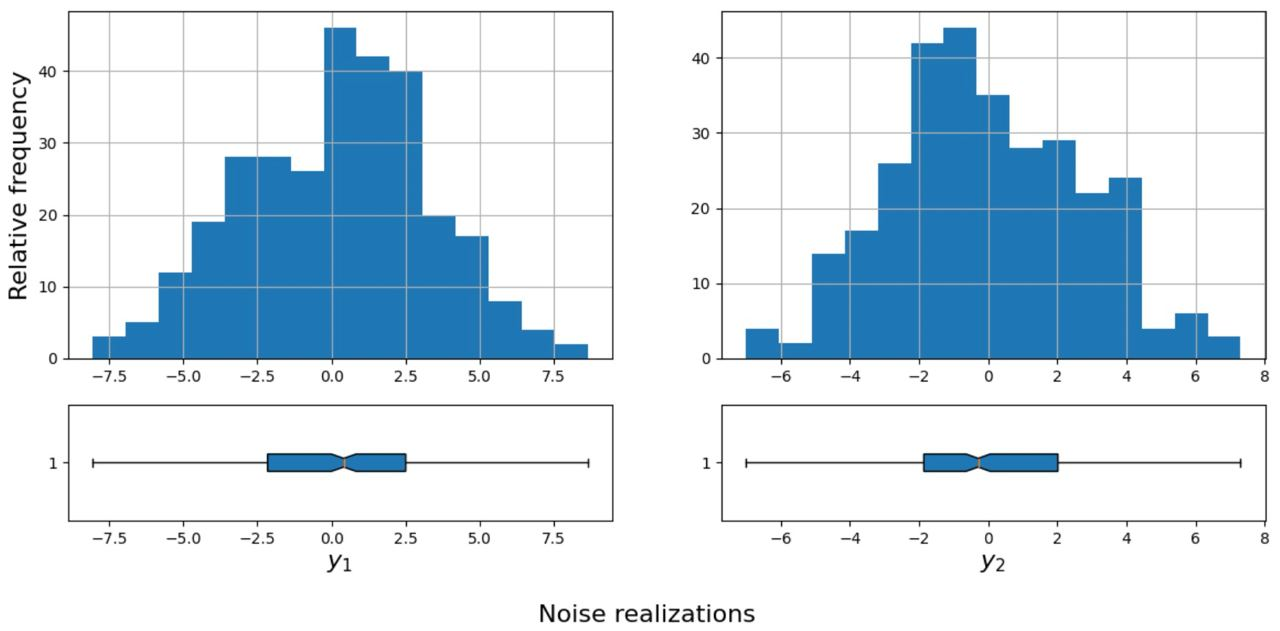
\includegraphics[width=0.9\columnwidth, height=\textheight,keepaspectratio]{figures/cvm/measurement_noise_normal.jpg}}
\label{fig:cvm_measurement_noise_normal}
\end{figure}

\begin{figure}[!ht]
\centering
\caption{(CVM, Normal noise) The top four graphs show the one particular evolution of the normal and Cauchy scales \(\varepsilon_{y_1,t}, \varepsilon_{y_2,t}\), respectively. The bottom two represent the normal noise realizations.}
\subfloat{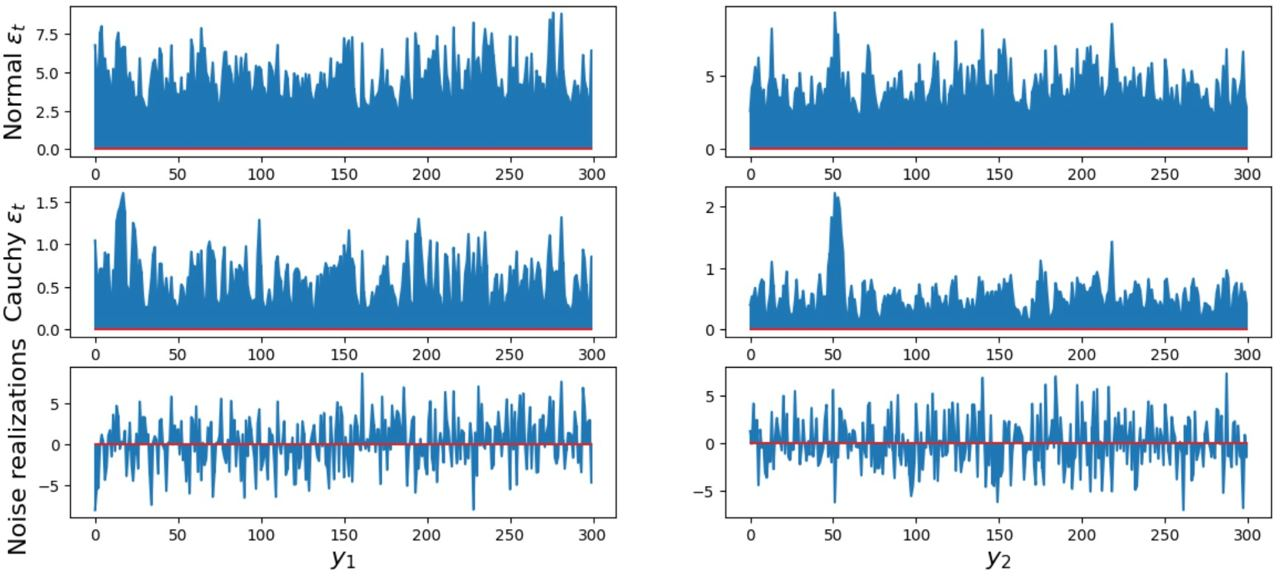
\includegraphics[width=0.9\columnwidth, height=\textheight,keepaspectratio]{figures/cvm/abc_scales_evolution_normal.jpg}}
\label{fig:cvm_abc_scales_evolution_normal}
\end{figure}

Again, as in the case of the PGM model, it can be argued that ABC filters can compete with filters requiring full knowledge of the measurement model, provided that these filters possess such knowledge. Given the context of full knowledge of the measurement model, it is still better to use KF, since of all the filters used in the experiment, it is the cheapest in terms of computational cost and the most accurate in terms of tracking.

\section{Example 3: Polar radar model}
The model that will be presented in this section is a modification of the CVM model, adding nonlinearity to it. Again, there is an object moving in 2D space, accurately described by equations (\ref{eq:cvm_equations}). But here it is assumed that the measurements of the object's motion will come directly from the radar. That is, in the context of this model, the measurements will be represented in a Polar coordinate system. 

The state evolution model, its noise term, and the corresponding covariance matrix remain identical to the CVM. As for the measurement model, it will look like this:

\begin{equation}
    \begin{aligned}
     y_t &=
    \begin{bmatrix}
        \rho_t \\ 
        \phi_t \\ 
        \dot{\rho}_t
    \end{bmatrix}
    = h(x_{t}) + \varepsilon_t,
    \end{aligned}
    \label{eq:prm_equations}
\end{equation}

\noident where

\begin{equation}
    \varepsilon_t \sim (0, R_t) \quad \text{with} \quad R &=
    r^{2}\cdot
    \begin{bmatrix}
        0.01 & 0.0 & 0.0 \\
        0.0 & 0.0001 & 0.0 \\
        0.0 & 0.0 & 0.01
    \end{bmatrix}.
\end{equation}

Where respectively the measurement \(y_t\) is a polar coordinate, which consists of the following elements: \(\rho\), \(\dot{\rho}\) are radius and velocity magnitude respectively and \(\phi\) is the angle in radians. Also, it was already clear that the function \(h(\cdot)\) is the function that converts 2D Cartesian position and velocity coordinates to Polar coordinates. This function is necessary because the prediction will be in Cartesian coordinates, but the measurement that comes from the radar is in Polar coordinates. The function itself looks as follows:

\begin{equation}
h\left(x\right)=\left(\begin{array}{c}
\rho \\
\phi \\
\dot{\rho}
\end{array}\right)=\left(\begin{array}{c}
\sqrt{x_1^2+x_2^2} \\
\arctan \left(x_2 / x_1\right) \\
\frac{x_1 v_1+x_2 v_2}{\sqrt{x_1^2+x_2^2}}
\end{array}\right).
\end{equation}

The set of filters that will take part in the experiment is already standard. Because of the use of the conversion function in the measurement equation, which is clearly non-linear, instead of the usual KF filter will be used its extended version. To use EKF in the measurement update cycle, one must linearize the function \(h(\cdot)\), that is, use a Taylor series expansion and take its first derivative. Since the work in the equation is done with a matrix, one can easily calculate its first-order derivative using the Jacobian matrix. That is, the linearization for the correction will look as follows:

\begin{equation}
    H = h'(x) = \left[\begin{array}{cccc}
\frac{x_1}{\sqrt{x_1^2+x_2^2}} & \frac{x_2}{\sqrt{x_1^2+x_2^2}} & 0 & 0 \\
-\frac{x_2}{x_1^2+x_2^2} & \frac{x_1}{x_1^2+x_2^2} & 0 & 0 \\
\frac{x_2\left(v_1 x_2-v_2 x_1\right)}{\left(x_1^2+x_2^2\right)^{3 / 2}} & \frac{x_1\left(v_2 x_1-v_1 x_2\right)}{\left(x_1^2+x_2^2\right)^{3 / 2}} & \frac{x_1}{\sqrt{x_1^2+x_2^2}} & \frac{x_2}{\sqrt{x_1^2+x_2^2}}
\end{array}\right]
\end{equation}

And as in the previous examples in this chapter, based on the assumption that the model is correctly specified, the noise terms belong to following normal distributions:

\begin{equation}
\begin{aligned}
w_t &\sim \mathcal{N}(0, Q_t), \\
\varepsilon_t &\sim \mathcal{N}(0, R_t).
\end{aligned}
\end{equation}

\paragraph*{Initialization} The model initialization parameters will not differ from what was set in the CVM. The initial parameters are \(x_0=[0,0,1,-1] \), \(dt=1\), \(r=3\), \(q=\sqrt{5}\), the length of the series is 300 samples. As for the EKF filter: \(x_0 = [1,1,1,1]\) and \(P^{-} = 10000 I_{4 \times 4}\). An initial set of 1000 particles is randomly sampled from \(\mathcal{N}\left(\left[1,1,1,1\right], 10 I_{4 \times 4} \right)\) and used in all SMC filters. The setting of the ABC filters also remain unchanged from previous experiments: the HPR value \(p = 0.95\) in order to cover \(90\%\) of pseudo-measurements. An experiment with 100 repetitions was conducted to obtain representative results.

\paragraph*{Charts and analysis}
The analysis will begin again with a consideration of MSE values, which are represented by Figure \ref{fig:pgm_mse_boxplot_normal} and Table \ref{table:prm_mse_normal}, where the first figure shows the final results after 100 experiment runs and the second figure shows the averaged values. Also with regard to box plots, for better readability and because of the longest whiskers, the results for the ABC filter with Cauchy kernel for the state variables \(x_1\) and \(x_2\) are put on a separate graph (in the middle).

Given the rather high non-linearity of the measurement model, almost all filters showed far from outstanding results, especially when it comes to tracking \(x_1\) and \(x_2\). The best of all were, as throughout this chapter, the EKF and PF filters. This time the PF filter performed worse than the EKF. From the Figure \ref{fig:pgm_mse_boxplot_normal} with box plots, one can see that PF was sometimes very inaccurate when tracking \(x_1\) and \(x_2\). This is also confirmed by the Table \ref{table:prm_mse_normal} with averaged values. As for the ABC filters, they in particular experienced great difficulty in keeping track of the state variables \(x_1\) and \(x_2\). The final MSE values of some experiment runs were so high that they also affected the averaged values in the Table \ref{table:prm_mse_normal}. If ABC with a normal kernel has a critical averaged MSE value only when tracking the variable \(x_1\), then a filter with a Cauchy kernel has a huge averaged MSE for both \(x_1\) and \(x_2\). As for tracking \(v_1\) and \(v_2\), all filters showed generally acceptable results. Returning to the ABC filters, it can be said that this time they did not prove to be competitive, especially the filter with the Cauchy kernel showed the worst results.

\begin{figure}[!ht]
\centering
\caption{(PRM, Normal noise) Box plots showing final MSE values for all state variables $x_1$, $x_2$, $v_1$ and $v_2$ of 100 repeated experiments. The boxes show medians, upper and lower quartiles. The length of the whiskers is defined as 1.5 times the interquartile range. The outliers are not displayed.}
\subfloat{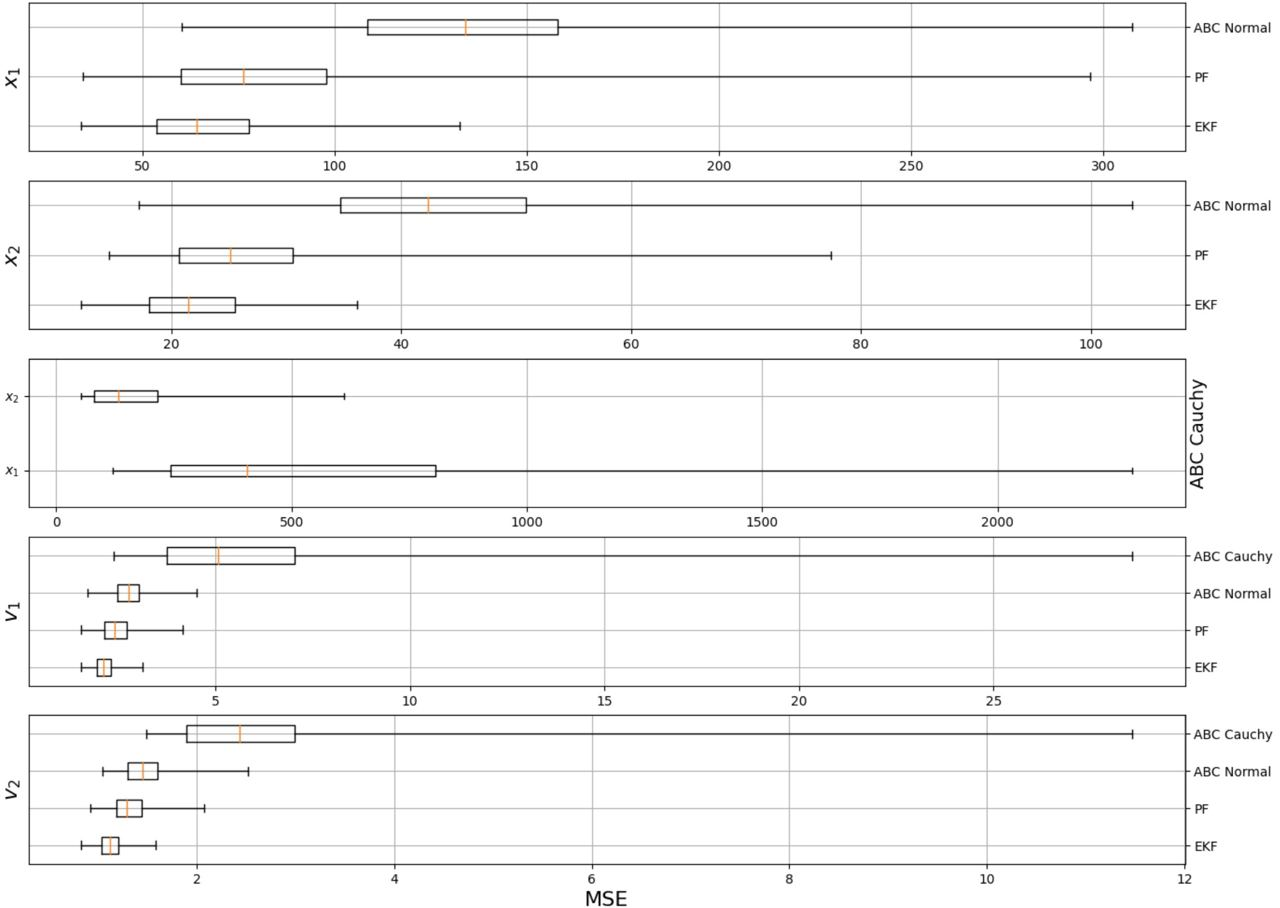
\includegraphics[width=0.9\columnwidth, height=\textheight,keepaspectratio]{figures/prm/mse_boxplot_normal.jpg}}
\label{fig:prm_mse_boxplot_normal}
\end{figure}

\begin{table}[h!]
\centering
\begin{tabular}{ |p{2cm}|p{2cm}|p{2cm}|p{2cm}|p{2cm}|}
 \hline 
  & $x_1$ & $x_2$ & $v_1$ & $v_2$ \\
 \hline \hline
 EKF & 66.235 & 21.636 & 2.161 & 1.122  \\
 PF & 81.980  & 26.763 & 2.433 & 1.333 \\
 ABC Normal & 140.496 & 44.511 & 2.846 & 1.474 \\
 ABC Cauchy & 957.038 & 261.612 & 5.908 & 2.703 \\
 \hline
\end{tabular}
\caption{(PRM, Normal noise) The final MSE values for all state variables $x_1$, $x_2$, $v_1$ and $v_2$ averaged over 100 runs}
\label{table:prm_mse_normal}
\end{table}

Also on the Figures \ref{fig:prm_measurement_noise_normal} and \ref{fig:prm_abc_scales_evolution_normal}, one can take a closer look at one particular realization of measurement noises \(\varepsilon_{y_1,t}\), \(\varepsilon_{y_2,t}\), \(\varepsilon_{y_3,t}\), and also the resulting settings of kernels. In terms of kernel tuning, on the example of these data it can be stated that the ABC filters reflects well the noise evolution. It is worth expecting that the responses to significant values of the noise terms will be more evident in the next chapter.

\begin{figure}[!ht]
\centering
\caption{(PRM, Normal noise) One particular normal noise realizations \(\varepsilon_{y_1,t}\), \(\varepsilon_{y_2,t}\) and \(\varepsilon_{y_3,t}\). Relative frequency histograms and box plots. Each box shows the median, upper and lower quartiles. The length of
the whiskers is defined as 1.5 times the interquartile range. Dots closer to the edges of the box represent
outliers.}
\subfloat{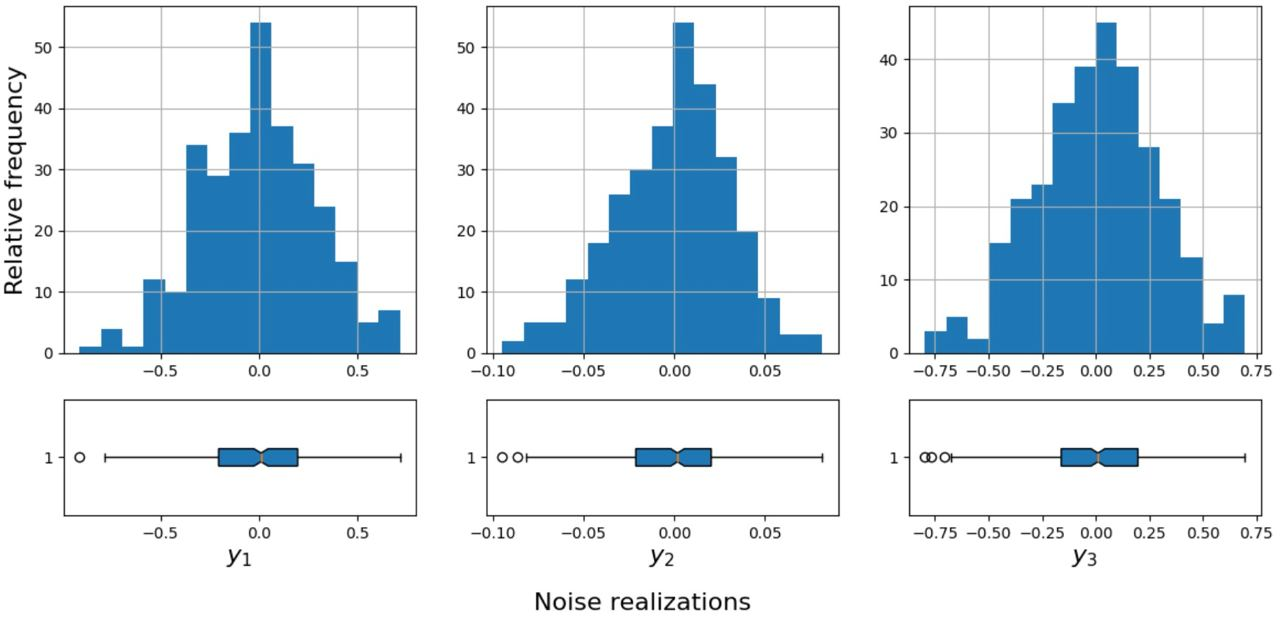
\includegraphics[width=0.9\columnwidth, height=\textheight,keepaspectratio]{figures/prm/measurement_noise_normal.jpg}}
\label{fig:prm_measurement_noise_normal}
\end{figure}

\begin{figure}[!ht]
\centering
\caption{(PRM, Normal noise) The top four graphs show the one particular evolution of the normal and Cauchy scales \(\varepsilon_{y_1,t}, \varepsilon_{y_2,t}\), and \(\varepsilon_{y_3,t}\), respectively. The bottom three represent the normal noise realizations.}
\subfloat{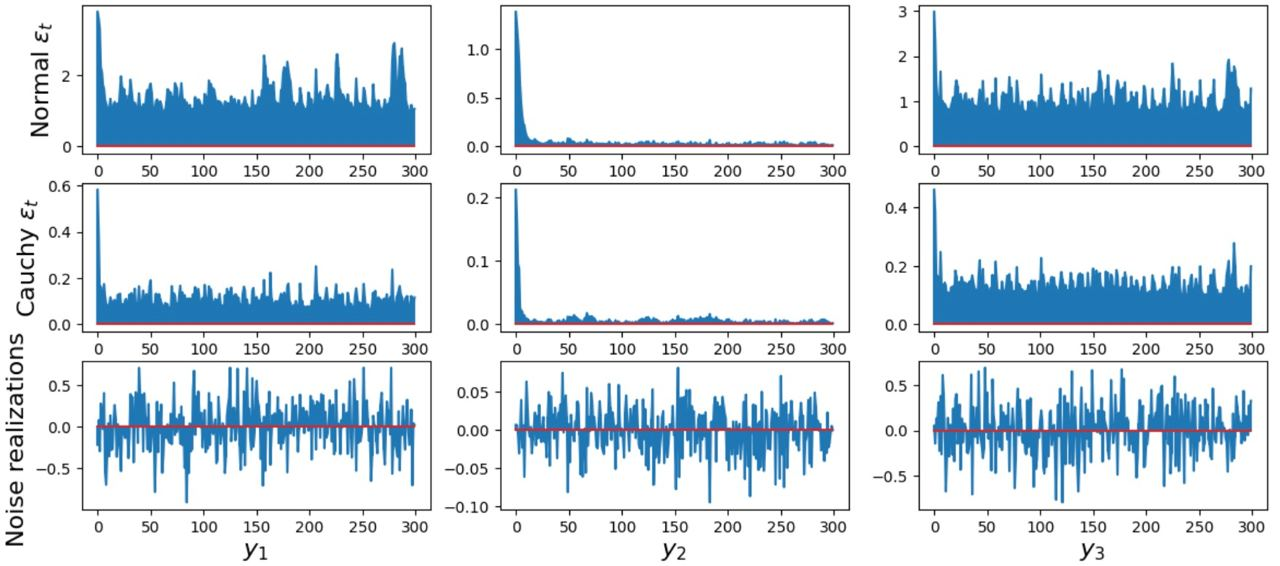
\includegraphics[width=0.9\columnwidth, height=\textheight,keepaspectratio]{figures/prm/abc_scales_evolution_normal.jpg}}
\label{fig:prm_abc_scales_evolution_normal}
\end{figure}

\section{Experiments conclusion}
In general, it can be summarized that with full knowledge of the measurement model, it does not make much sense to use ABC filters, which, in most cases, show pretty good results but are still inferior to PF and KF filters. It is also worth considering that in terms of computational cost, they are insignificantly but still more expensive.

As for the KF filter, having a well-specified model and guaranteed linearity, it can be safely declared that it is the best linear estimator, which is confirmed by the results of the experiments. Its extended version also showed itself from the best side. The PF filter showed itself almost on par with KF and EKF, and sometimes EKF was even inferior to it. However, it should be kept in mind that to use PF, which performs on par or even better than KF or EKF, one will have to sacrifice the use of a large number of particles, which directly affects the computational complexity. It is also worth noting that in the case of EKF, when one of the steps, either prediction or update, is highly nonlinear, EKF will have relatively not the best efficiency. In addition, the quite high computational cost of computing the Jacobian matrix is worth considering when using EKF.

To summarize, once again, it can be said that, if the condition that the measurement model is completely known and both state and measurement equations are linear with zero mean Gaussian noise is satisfied, then it is best to use the standard KF filter. In the case of nonlinearity, it would be better to use the PF filter.